$server.cpp$ es la implementación del ciclo principal del servidor. Su función es establecer las conexiones con los jugadores y controladores y atenderlos mediante dos funciones:

\begin{itemize}
	\item void atender\_jugador(int i): Dado un mensaje del jugador i, ejecuta el comando pedido y envía la respuesta y los eventos pendientes para este jugador.
	\item void void atender\_controlador(): Dado un mensaje del controlador, ejecuta el comando y envía la respuesta.
\end{itemize}

Mediante la creación de varios threads se buscará:

\begin{itemize}
	\item Permitir que múltiples jugadores puedan conectarse al $backend$ de forma simultánea.
	\item Permitir que uno o varios controladores se conecten al backend en cualquier momento sin importar el estado del juego y puedan obtener los puntajes de los jugadores con el comando Get\_Scores.
\end{itemize}

Para ello realizamos diversas modificaciones en el código del server previsto. Disponemos de un $main$ $thread$ encargado de orquestar todo el sistema distribuyendo trabajos a otros $threads$. A continuación presentamos un esquema ilustrativo del funcionamiento:

\begin{figure}[H]
\centering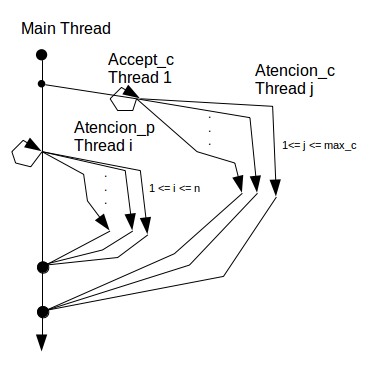
\includegraphics[scale=0.7]{imgs/server.png}
\caption{Esquema del funcionamiento del server.}
\end{figure}

Cuando un jugador quiere conectarse al juego el $main$ $thread$ realiza las siguientes operaciones:

\begin{itemize}
	\item[1] Espera que la conexión sea aceptada por el servidor.
	\item[2] Crea un nuevo $thread$ que atiende al jugador entrante mediante la función $atencion\_p$ (Habrá tantos $threads$ como jugadores haya en el sistema). El jugador será atendido hasta que finalice el juego.
	\item[3] Cuando finaliza el juego, el $thread$ encargado de atender al jugador termina avisándole al $main$ $thread$.
\end{itemize}

Pseudocódigo:

\begin{algorithm}[H]
\caption{Jugador}\label{ej1}
\begin{algorithmic}[1]
\Procedure{Jugador}{}
	\State $pthread\_t \ threads[MAX\_JUGADORES]$ 
	\State $int \ tids[MAX\_JUGADORES]$
	\For{jugador = 0 to n}
		\State accept(jugador)
		\State $pthread\_create(\&threads[i],NULL,atencion\_p,\&tids[jugador])$
	\EndFor
\EndProcedure
\end{algorithmic}
\end{algorithm}

\begin{algorithm}[H]
\caption{atencion\_p}\label{ej1}
\begin{algorithmic}[1]
\Procedure{atencion\_p}{jugador}
	\State $bool$ $sale$ $=$ $false$ 
	\While {$!sale$}
		\State atender\_jugador(jugador)
		\State sale = model->termino()
	\EndWhile
	\State $pthread\_exit(NULL)$
\EndProcedure
\end{algorithmic}
\end{algorithm}

El funcionamiento es similar en el caso de los controladores. El $main$ $thread$ crea un $thread$ (thread\_atencion\_controladores) encargado de esperar y aceptar conexiones entrantes. Este $thread$ lanza un nuevo $thread$ cada vez que llega un controlador y ejecuta la función $atencion\_c$. Pseudocódigo:

\begin{algorithm}[H]
\caption{Controlador}\label{ej1}
\begin{algorithmic}[1]
\Procedure{Controlador}{}
	\State $pthread\_t  \ thread\_atencion\_controladores$
	\State $pthread\_create(\&thread\_atencion\_controladores,NULL,accept\_c,NULL)$
\EndProcedure
\end{algorithmic}
\end{algorithm}

\begin{algorithm}[H]
\caption{accept\_c}\label{ej1}
\begin{algorithmic}[1]
\Procedure{accept\_c}{}
	\State $pthread\_t \ control\_threads[MAX\_CONTROLADORES]$
	\State $int \ c\_tids[MAX\_CONTROLADORES]$
	\For{controlador = 0 to MAX\_CONTROLADORES}
		\State accept(controlador)
		\State $pthread\_create(\&control\_threads[controlador],NULL,atencion\_c,\&c\_tids[controlador])$
	\EndFor
\EndProcedure
\end{algorithmic}
\end{algorithm}

\begin{algorithm}[H]
\caption{atencion\_c}\label{ej1}
\begin{algorithmic}[1]
\Procedure{atencion\_c}{controlador}
	\State atender\_controlador(controlador);
	\State close(s\_controladores[controlador]);
	\State $pthread\_exit(NULL)$
\EndProcedure
\end{algorithmic}
\end{algorithm}

Una vez que todos los $threads$ encargados de atender a los jugadores y controladores finalizan, el $main$ $thread$ termina su ejecución. Esto se logra gracias al join. Hacer join de un $thread$ significa que este espera a los demas $threads$ para finalizar:

\begin{algorithm}[H]
\caption{Join}\label{ej1}
\begin{algorithmic}[1]
\Procedure{Join}{}
	\For{int tid = 0 to n}
		\State $pthread\_join(threads[tid], NULL)$
	\EndFor
	\For{int tid = 0 to MAX\_CONTROLADORES}
		\State $pthread\_join(control\_threads[tid], NULL)$
	\EndFor
\EndProcedure
\end{algorithmic}
\end{algorithm}
